\documentclass[5pt]{beamer}

\usepackage[english]{babel}
\usepackage[utf8]{inputenc}
\usepackage{graphicx}
\usepackage{subcaption}
\usepackage{hyperref}
\usepackage{multicol}
\usepackage{listings}

\usepackage{listings}
\usefonttheme{professionalfonts}
\setbeamertemplate{itemize items}[ball]

\usepackage{enumitem,xcolor}
\definecolor{lightgray}{RGB}{220 220 220}

\lstset{language=C++,tabsize=4, literate={é}{{\'e}}1 {è}{{\`e}}1 {ê}{{\^e}}1 {à}{{\`a}}1, stringstyle=\color{red}, keywordstyle=\color{blue}, identifierstyle=\color{black}}%{É}{{\'E}}1

\newcommand{\code}[1]{\colorbox{lightgray}{\lstinline~#1~}}

\usetheme{Darmstadt}
\definecolor{clearblueifnti}{RGB}{24,116,220}
\setbeamercolor{title}{use=structure,bg=clearblueifnti,fg=white}

\makeatletter
\setbeamertemplate{title page}{
  \vbox{}
  \vfill
  \begingroup
    \centering\hspace{2cm}
    \begin{minipage}{.7\textwidth}
    \begin{beamercolorbox}[sep=8pt,center,shadow=true,rounded=true]{title}
      \usebeamerfont{title}\inserttitle\par%
      \ifx\insertsubtitle\@empty%
      \else%
        \vskip0.25em%
        {\usebeamerfont{subtitle}\usebeamercolor[fg]{subtitle}\insertsubtitle\par}%
      \fi%     
    \end{beamercolorbox}%
    \end{minipage}

    \vskip2.8em\par
    \begin{minipage}{\textwidth}
    \begin{beamercolorbox}[sep=8pt,center]{author}
      \usebeamerfont{author}\insertauthor
    \end{beamercolorbox}
    \end{minipage}

    \begin{minipage}{\textwidth}
    \begin{beamercolorbox}[sep=8pt,center]{institute}
      \usebeamerfont{institute}\insertinstitute
    \end{beamercolorbox}
    \end{minipage}

    \begin{minipage}{\textwidth}
    \begin{beamercolorbox}[sep=8pt,center]{date}
      \usebeamerfont{date}\insertdate
    \end{beamercolorbox}
    \end{minipage}
    \vskip0.5em
    {\usebeamercolor[fg]{titlegraphic}\inserttitlegraphic\par}
  \endgroup
  \vfill
}
\makeatother

\title{PROJET :Présentation du projet IMMO-ADJA }
%\subtitle[UI]{Gestion des biens immobiliers}
\institute{IFNTI S4}
\author{Presenté par : KUMENA M'BA Roland \& OGBONE INOUSSA Chérifa \& SOKA Dissima}

\date{\today}

\setbeamertemplate{footline}
{
  \hbox{
  \begin{beamercolorbox}[wd=.3\paperwidth,ht=2.25ex,dp=1ex,center]{author in head/foot}
    \usebeamerfont{author in head/foot}\insertshortauthor
  \end{beamercolorbox}
  \begin{beamercolorbox}[wd=.6\paperwidth,ht=2.25ex,dp=1ex,center]{date in head/foot}
    \usebeamerfont{date in head/foot}\insertshortsubtitle{} : \inserttitle{} - \insertshortinstitute{} - \insertdate
  \end{beamercolorbox}
  \begin{beamercolorbox}[wd=.1\paperwidth,ht=2.25ex,dp=1ex,center]{title in head/foot}
    \usebeamerfont{title in head/foot}\insertframenumber{} / \inserttotalframenumber
  \end{beamercolorbox}}
}

\usebackgroundtemplate{
\includegraphics[width=\paperwidth,height=\paperheight]{CharteGraphiquePresentationCorps}}

\begin{document}

{
\setbeamertemplate{headline}{\vskip\headheight}
\setbeamertemplate{footline}{}
\usebackgroundtemplate{
\includegraphics[width=\paperwidth,height=\paperheight]{CharteGraphiquePresentationPageDeGarde}}
\begin{frame}[plain]
	%\vspace{5cm}
	\titlepage\end{frame}
}

\begin{frame}{Table des matières}
	%\begin{multicols}{2}
	\tableofcontents
	%\end{multicols}
\end{frame}

{\AtBeginSection[]{
  \begin{frame}
  \vfill
  \centering
  \begin{beamercolorbox}[sep=8pt,center,shadow=true,rounded=true]{title}
    \usebeamerfont{title}\insertsection\par
  \end{beamercolorbox}
  \vfill
  \end{frame}
}



\section{ Introduction }
\begin{frame}[fragile]{Introduction}
\begin{block}{}
\begin{center}
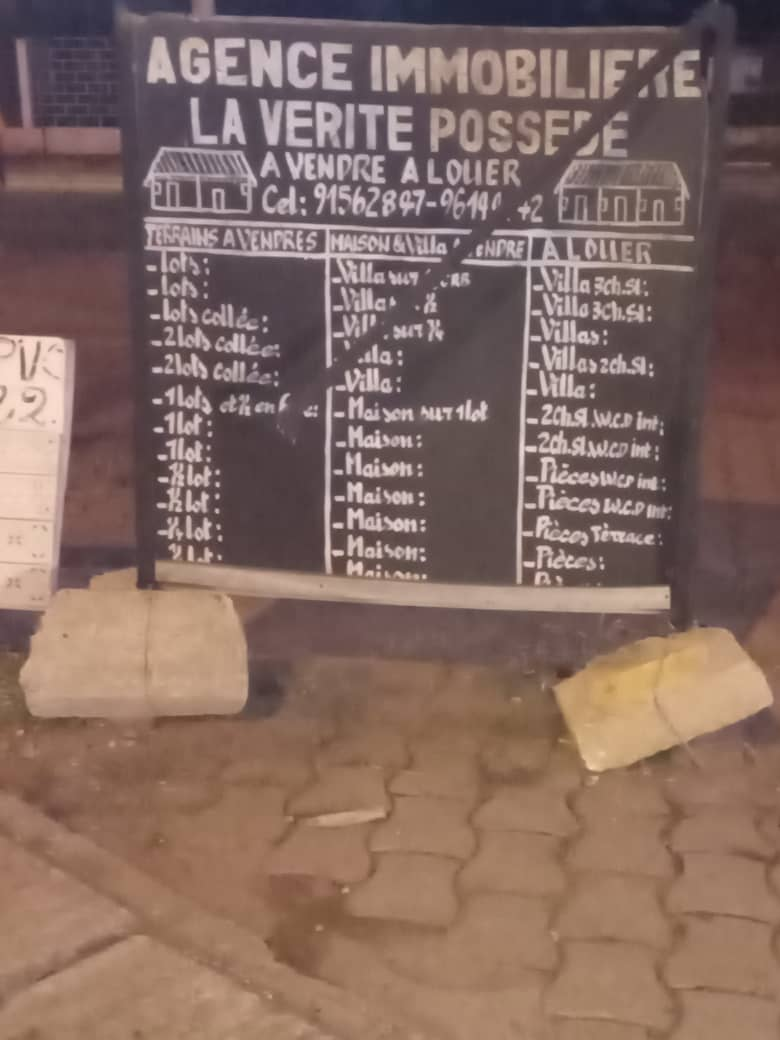
\includegraphics[scale=0.25]{Immo.jpeg}
\end{center}
\end{block}
\end{frame}

\section{ Analyse et Conception de l'application }
\begin{frame}[fragile]{Analyse et Conception de l'application}
\begin{block}{Diagramme de cas d'utilisation : Fonctionnement de l'application}

\begin{center}
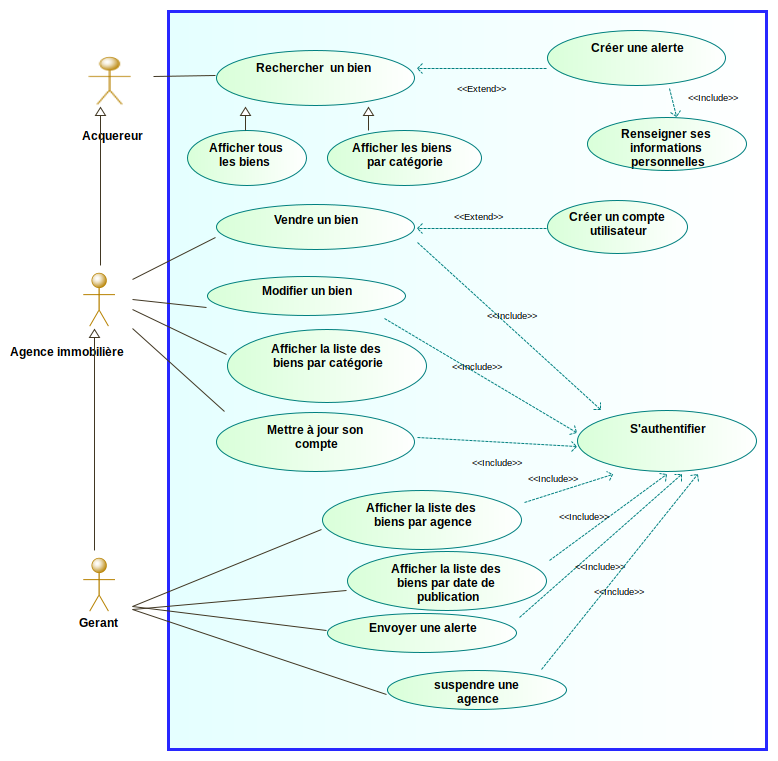
\includegraphics[scale=0.25]{diagramCas.png}
\end{center}
	\end{block}
\end{frame}
\begin{frame}[fragile]{Analyse et Conception de l'application}
\begin{block}{Diagramme de classe}

\begin{center}
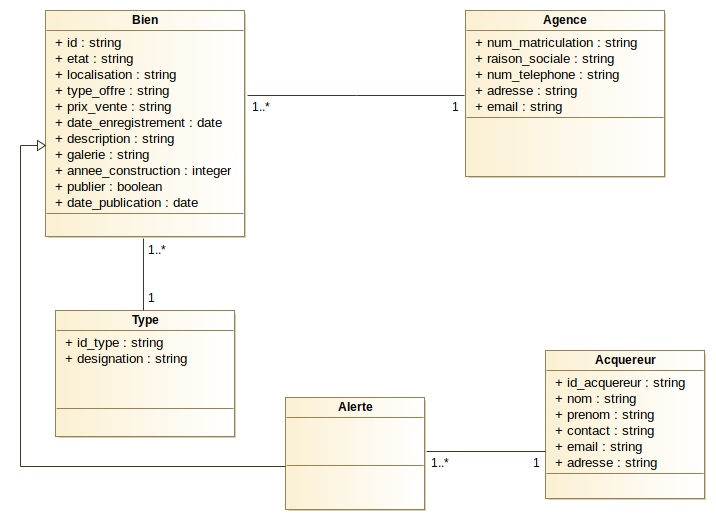
\includegraphics[scale=0.25]{Diagramme_class.png}
\end{center}
	\end{block}
\end{frame}


\section{Démonstration technique}

\section{Difficultés rencontrées}
\begin{frame}[fragile]{Difficultés}
\begin{block}{Collecte d'information}
\end{block}
\begin{block}{Insuffisance de connaissance de la technologie utilisée }
\end{block}
\end{frame}

\section{Solutions}
\section{Technologies utilisées}
\section{Bilan du projet}
\section{MERCI POUR VOTRE ATTENTION}




\end{document}
